\section*{Задание 2}
    Найти решение следующей краевой задачи: 
    \[
        \left\{\begin{split}
            & \frac{1}{r} \frac{\partial}{\partial r} \left( r \frac{\partial u}{\partial r} \right) + \frac{1}{r^2} + \frac{\partial^2 u}{\partial r^2} = 0, \quad 4 < r < 5, \quad 0 < \varphi < 2\pi, \\
            & 2u|_{r=4} = 3, \quad 0 < \varphi < 2\pi, \\
            & u|_{r=5} = 5 - 2.3 \sin \varphi, \quad 0 < \varphi < 2\pi. \\
        \end{split} \right.
    \]
    Ищем решение в виде \( u(r, \varphi) = P(r) \cdot \Phi(\varphi) \).
    \[
        \frac{1}{r} \left( r P' \Phi \right)' = - \frac{1}{r^2} P \Phi''
        \quad \Rightarrow \quad
        \frac{r\left(r P'\right)'}{P} = - \frac{\Phi''}{\Phi} = \mu^2
    \]
    \begin{enumerate}
        \item Решим задачу Штурма-Лиувилля для второго равенства.
        \[
            \left\{\begin{split}
                & \Phi'' + \mu^2 \Phi = 0, \\
                & \Phi(\varphi) = \Phi(\varphi + 2\pi).
            \end{split}\right.
            \Rightarrow
            \Phi(\varphi) = C_1 \sin (\mu \varphi) + C_2 \cos (\mu \varphi) 
        \]
        \[
            C_1 \sin (\mu \varphi) + C_2 \cos (\mu \varphi) = C_1 \sin \left(\mu (\varphi+2\pi)\right) + C_2 \cos \left(\mu (\varphi+2\pi)\right)
        \]
        Такое происходит только когда \( \mu_n = n, n \in \mathbb{N}_0 \). \( (n = 0,1,2,\dots) \) Значит решение выглядит так:
        \(
            \Phi_n = A_n \sin (\varphi n) + B_n \cos (\varphi n)
        \).
        \item Найдём решение для первого равенства.
        \[
            r\left( r P' \right)' - \mu_n^2 P = 0.
        \]
        Если \( n = 0 \), то 
        \[
            P_0 = A_0 + B_0 \ln r.
        \]
        Задача в кольце, поэтому \(P_0\) остаётся в таком виде.
        \[
            P_n^{(1)}(r) = r^n, \quad P_n^{(2)}(r) = \frac{1}{r^n}.
        \]
        Задача в кольце, значит выбираем линейную комбинацию решений:
        \[ P_n(r) = C_n^{(1)} r^n + C_n^{(2)} \frac{1}{r^2}. \]
    \end{enumerate}

    Заменяем коэффициенты \( C_n^{(1)} A_n = A_n, \, C_n^{(1)} B_n = B_n, \, C_n^{(2)} A_n = C_n, \, C_n^{(2)} B_n = D_n \) и получаем:
    \[
        \begin{split}
            & u(r, \varphi) = \sum_{n=0}^{\infty} u_n(r, \varphi) = A_0 + B_0 \ln r + \sum_{n=1}^{\infty} r^n \left( A_n \sin (\varphi n) + B_n \cos (\varphi n) \right) + \\
            & + \sum_{n=1}^{\infty} \frac{1}{r^n} \left( C_n \sin (\varphi n) + D_n \cos (\varphi n) \right)
        \end{split}
    \]

    Подставим в граничные условия:
    \[
        \left\{\begin{split}
            & 2 u|_{r=4} = 2A_0 + 2B_0 \ln 4 + 2\sum_{n=1}^{\infty} 4^n \left( A_n \sin (\varphi n) + B_n \cos (\varphi n) \right) + \\
            & + \sum_{n=1}^{\infty} \frac{1}{4^n} \left( C_n \sin (\varphi n) + D_n \cos (\varphi n) \right) \equiv 3, \\[10pt]
            & u|_{r=5} = A_0 + B_0 \ln 5 + \sum_{n=1}^{\infty} 5^n \left( A_n \sin (\varphi n) + B_n \cos (\varphi n) \right) + \\
            & + \sum_{n=1}^{\infty} \frac{1}{5^n} \left( C_n \sin (\varphi n) + D_n \cos (\varphi n) \right) \equiv 5 - 2.3 \sin \varphi.
        \end{split}\right.
    \]

    Сопоставим коэффициенты и найдём их.
    \begin{enumerate}
        \item При константах:
            \[
                \left\{ \begin{split}
                    & 2A_0 + 2B_0 \ln4 = 3, \\
                    & A_0 + B_0 \ln5 = 5.
                \end{split}\right.
                \Rightarrow
                \left\{ \begin{split}
                    & B_0 = \frac{7}{2(\ln5 - \ln 4)}, \\
                    & A_0 = 5 - \frac{7 \ln 5}{2(\ln 5 - \ln 4)} = \frac{3 \ln5 - 10 \ln 4}{2(\ln5 - \ln4)}
                \end{split}\right.
            \]
        \item При \( n = 1 \):
            \[
                \left\{ \begin{split}
                    & 2 \cdot 4 A_1 + 2\cdot\frac{1}{4} C_1 = 0, \\
                    & 5 A_1 + \frac{1}{5} C_1 = -2.3.
                \end{split}\right.
                \Rightarrow
                \left\{ \begin{split}
                    & A_1 = -\frac{23}{18}, \\
                    & C_1 = \frac{184}{9}
                \end{split}\right.
            \]
        \item Все остальные коэффициенты равны нулю.
    \end{enumerate}

    \noindent \textit{Ответ:} \( u(r, \varphi) = \frac{3 \ln5 - 10 \ln 4}{2(\ln5 - \ln4)} + \frac{7}{2(\ln5 - \ln 4)} \ln r -\frac{23}{18} r \sin \varphi + \frac{184}{9} \frac{1}{r} \sin \varphi \).

    \begin{figure}[H]
        \centering
        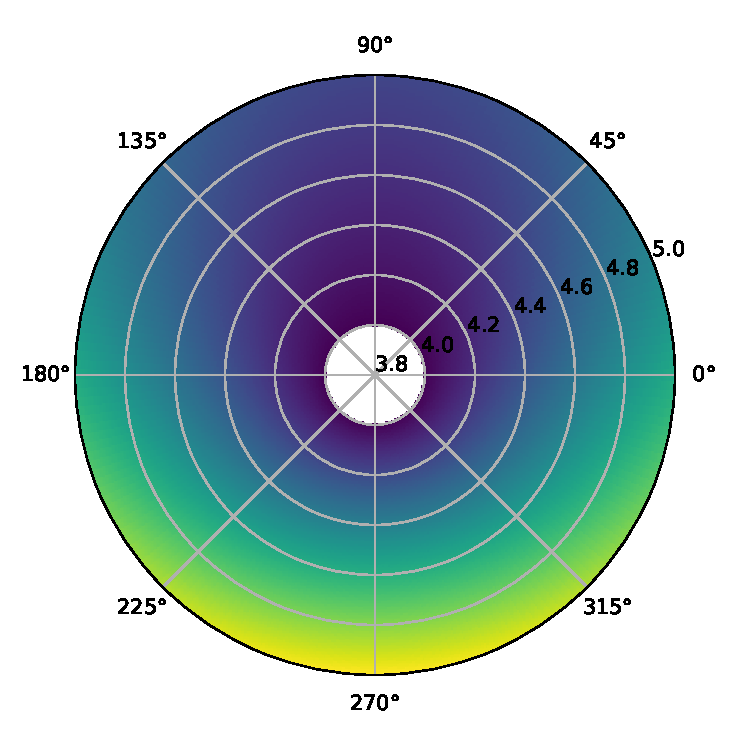
\includegraphics[width=14cm]{p2.pdf}
    \end{figure}

